% !TEX TS-program = pdflatex
% !TEX encoding = UTF-8 Unicode

% This is a simple template for a LaTeX document using the "article" class.
% See "book", "report", "letter" for other types of document.

\documentclass[11pt]{report} % use larger type; default would be 10pt

\usepackage[utf8]{inputenc} % set input encoding (not needed with XeLaTeX)

%%% Examples of Article customizations
% These packages are optional, depending whether you want the features they provide.
% See the LaTeX Companion or other references for full information.

%%% PAGE DIMENSIONS
\usepackage{geometry} % to change the page dimensions
\geometry{a4paper} % or letterpaper (US) or a5paper or....
% \geometry{margin=2in} % for example, change the margins to 2 inches all round
% \geometry{landscape} % set up the page for landscape
%   read geometry.pdf for detailed page layout information

\usepackage{graphicx} % support the \includegraphics command and options

% \usepackage[parfill]{parskip} % Activate to begin paragraphs with an empty line rather than an indent

%%% PACKAGES
\usepackage{booktabs} % for much better looking tables
\usepackage{array} % for better arrays (eg matrices) in maths
\usepackage{paralist} % very flexible & customisable lists (eg. enumerate/itemize, etc.)
\usepackage{verbatim} % adds environment for commenting out blocks of text & for better verbatim
\usepackage{subfig} % make it possible to include more than one captioned figure/table in a single float
% These packages are all incorporated in the memoir class to one degree or another...

%%% HEADERS & FOOTERS
\usepackage{fancyhdr} % This should be set AFTER setting up the page geometry
\pagestyle{fancy} % options: empty , plain , fancy
\renewcommand{\headrulewidth}{0pt} % customise the layout...
\lhead{}\chead{}\rhead{}
\lfoot{}\cfoot{\thepage}\rfoot{}

%%% SECTION TITLE APPEARANCE
\usepackage{sectsty}
\allsectionsfont{\sffamily\mdseries\upshape} % (See the fntguide.pdf for font help)
% (This matches ConTeXt defaults)

%%% ToC (table of contents) APPEARANCE
\usepackage[nottoc,notlof,notlot]{tocbibind} % Put the bibliography in the ToC
\usepackage[titles,subfigure]{tocloft} % Alter the style of the Table of Contents
\renewcommand{\cftsecfont}{\rmfamily\mdseries\upshape}
\renewcommand{\cftsecpagefont}{\rmfamily\mdseries\upshape} % No bold!

%%% END Article customizations

%%% The "real" document content comes below...
\setcounter{tocdepth}{3}

\title{NaoCar}
\author{Samuel Olivier\and
Gaël du Plessix\and
Melvin Laplanche\and
Loick Michard}

%\date{} % Activate to display a given date or no date (if empty),
         % otherwise the current date is printed 

\begin{document}
\maketitle
\tableofcontents

\chapter{Contexte}
	\section{Bilan de la technologie}
		\subsection{La robotique aujourd'hui}
			Depuis quelques années, la recherche en matière de robotique a tendance à évoluer en direction des robots humanoïdes.
			En effet, les chercheurs visent à construire des robots effectuant toutes les actions qu'un humain est capable de réaliser.
			Notamment marcher sur deux jambes, attraper des objets, parler, communiquer ou même conduire...\\
			La recherche en robotique a pour objectif final d'assister l'humain dans les taches quotidiennes, voire de le remplacer.
			\subsubsection{Asimo}
				\begin{figure}[htb]
				\centering
				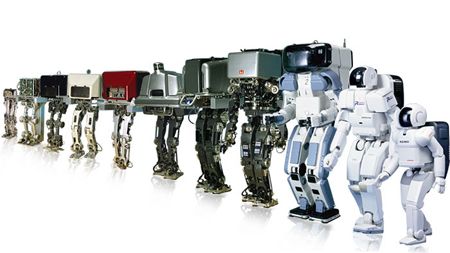
\includegraphics[width=0.8\textwidth]{asimo-history.jpg}
				\caption{Histoire de l'Asimo}
				\label{fig:asimo}
				\end{figure}
				\newpage
				L'Asimo représente la pointe de la robotique en matière d'humanoide.
				Il est capable de courir jusqu'à 9 km/h tout en changeant sa trajectoire, monter et descendre les escaliers, détecter les mouvements des objets, garder son équilibre...
			\subsubsection{Google Car}
				\begin{figure}[htb]
				\centering
				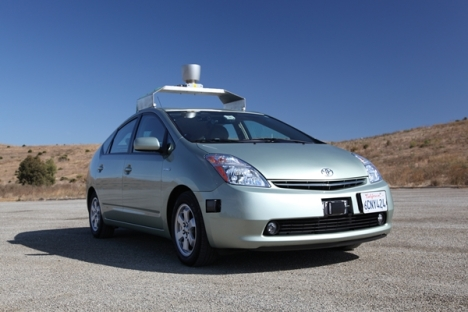
\includegraphics[width=0.8\textwidth]{google-car.jpeg}
				\caption{Google Car}
				\label{fig:google-car}
				\end{figure}
				La Google car est une des dernières innovation de Google en terme de recherche et de développement.
				Elle intègre une intelligence artificielle capable de conduir en autonomie dans des conditions très variés, de s'intégrer dans le trafic, de prévoir les actions des autres usagers... Elle a déjà été autorisé à conduire en autonomie dans plusieurs états Américains et parcourue plusieurs milliers de kilometres.
		\newpage
		\subsection{NAO}
			\begin{figure}[htb]
			\centering
			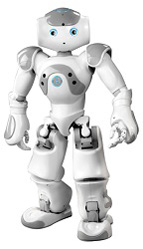
\includegraphics[scale=1]{nao2.jpg}
			\caption{NAO}
			\label{fig:nao}
			\end{figure}
			Nao est un robot humanoïde concu par la société Aldebaran pour etre entièrement programmable. Il dispose de 25 degrès de liberté, 1 accéléromètre, 2 gyromètres, et 2 caméras HD. Depuis le 15 août 2007, NAO remplace le chien robot Aibo de Sony comme plateforme standard de la RoboCup.
		\newpage
		\subsection{Kinect}
				\begin{figure}[htb]
				\centering
				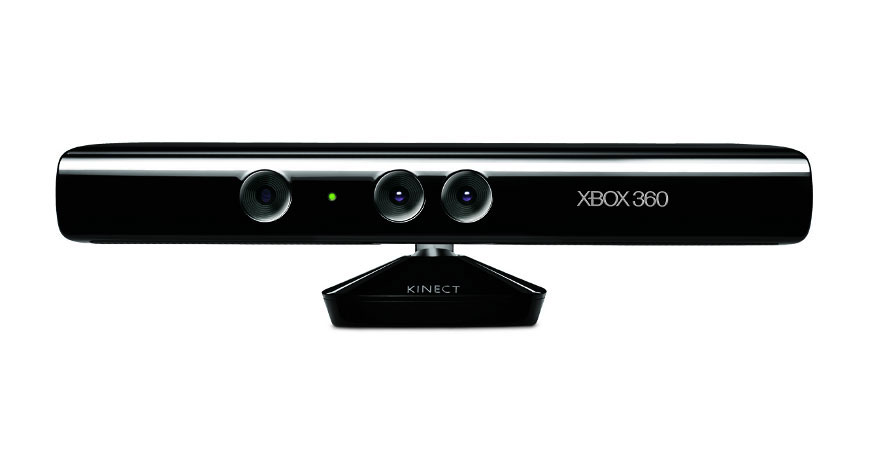
\includegraphics[width=0.8\textwidth]{kinect.jpg}
				\caption{Kinect}
				\label{fig:kinect}
				\end{figure}
				Kinect est une technologie développée par Microsoft permettant de controler un jeux vidéo sans utiliser de manette. Il est équipé d'une caméra et d'un capteur laser balayant l'environnement pour construire une image en profondeur de celui-ci. Gràce à ces deux capteurs, Kinect permet de connaitre la position dans l'espace des objects ainsi que détecter les mouvements des utilisateurs.
	\section{Un projet étudiant}
		\subsection{Epitech}
			\begin{figure}[htb]
			\centering
			
\includegraphics[width=0.8\textwidth]{epitech.png}
			\caption{Epitech}
			\label{fig:epitech}
			\end{figure}
			Epitech est une école d’informatique en 5 ans après le bac. Son modèle pédagogique novateur fournit aux étudiants trois qualités fondamentales : l’adaptabilité, l’auto-progression et le sens du projet.
		\subsection{PFA}
			Notre projet s'inscrit dans le cadre de la 3ème année à Epitech. Il se déroule pendant un an, incluant plannification, organisation, recherche de partenaires et développement du projet.\\
			
	\section{Une vision d'avenir}
			Le projet NaoCar se positionne dans la continuité des recherches actuelles, qui visent à amincir les frontières entre l'homme et la machine. En l'occurence, permettre à Nao de conduire une voiture pour enfant démontrerait de sa capacité à intéragir de manière transparente avec des objets conçus pour l'homme.
\chapter{Définition des objectifs}
	\section{Les objectifs techniques}
		\subsection{Contrôle et déplacement du robot}
			Le robot Nao doit être capable de manipuler les commandes de sa voiture afin d'effectuer les actions suivantes:
\begin{itemize}
\item Avancer
\item Reculer
\item Tourner à gauche
\item Tourner à droite
\end{itemize}
			Dans ce but, compte tenu de la configuration de son véhicule, Nao doit pouvoir:
\begin{itemize}
\item Actionner le levier de vitesse en position "avancer"
\item Actionner le levier de vitesse en position "reculer"
\item Tourner le guidon à gauche
\item Tourner le guidon à droite
\item Appuyer sur la pédale d'accélération
\end{itemize}
			Le robot doit pouvoir être contrôlé de manière très simple, via une interface proposant simplement les quatres actions avancer, reculer, tourner à gauche et tourner à droite.\\
			Ce contrôle devra pouvoir être effectué depuis un ordinateur et/ou un appareil mobile (smartphone/tablette) connecté sur le même réseau que le robot.
		\newpage
		\subsection{Intelligence artificielle: conduite autonome}
			\subsubsection{Conduite et reconnaissance de formes}
				Dans un premier temps, nao doit etre capable:
				\begin{itemize}
				\item De pouvoir conduire en suivant une ligne de couleur ou une piste spéciale
				\item De reconnaitre des formes simples pour permettre de s'arrêter au feu rouge par exemple
				\item De détecter les obstacles, s'arrêter, voire les contourner grâce au Kinect
				\end{itemize}
			\subsubsection{Vers une conduite en totale autonomie}
				Dans un second temps, Nao doit pouvoir conduire dans un espace connu en totale autonomie.
				Il doit pouvoir suivre un itinéraire donné, éviter les obstacles, et se repérer dans un environnement en 3 dimensions.\\
				Il devra utiliser des techniques de localisation pour palier au problème du déterminisme de ses actions, comme les filtres particulaires.
			\subsubsection{Plannification et modélisation}
				Enfin, Nao pourra évoluer dans un monde inconnu. Il devra être capable de parcourir un tout nouvel environnement en dressant une carte en 2 ou 3 dimensions de celui-ci. Il devra pour cela utiliser des techniques de cartographie et de localisation simultanées (SLAM).\\
				Grâce à cela, Nao sera en mesure de modeliser et de parcourir l'ensemble d'un environement totalement inconnu et non déerministe.
		\subsection{Matériel}
			Dans un premier temps, le véhicule utilisé sera une voiture pour enfant légèrement modifiée afin de pouvoir être pilotée par Nao. La voiture retenue se déplace à une vitesse de 3 km/h et dispose d'un faible angle de braquage. Cette première solution permettra de concevoir les solutions logicielles de pilotage et de conduite autonome afin de réaliser un premier prototype.\\
			Dans une seconde partie, l'objectif est de réaliser un véhicule spécialement dédié au Nao, lui permettant de se déplacer plus vite et disposant d'un meilleur angle de braquage.
	\section{Communication autour du projet}
		\subsection{Évènements}
			\subsubsection{Foire exposition de Montpellier}
				\begin{figure}[htb]
				\centering
				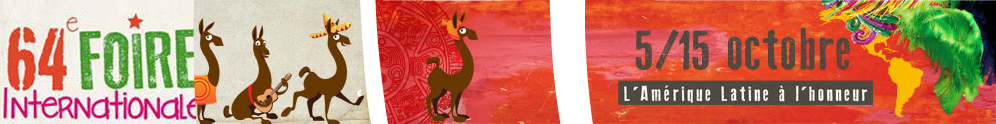
\includegraphics[width=1\textwidth]{foire-expo.png}
				\caption{Foire Expo Montpellier}
				\label{fig:Foire Expo Montpellier}
				\end{figure}
				La foire expositons internationale de Montpellier est un évènement de choix pour présenter le projet NaoCar au public pour la première fois. Installée au Parc des Expositions de Montpellier, elle dispose d'un espace d'exposition de 88 000 m\textsuperscript{2}, réunissant 1000 exposants durant 11 journées.
			\subsubsection{Montpellier In Game}
				\begin{figure}[htb]
				\centering
				
\includegraphics[width=1\textwidth]{mig.png}
				\caption{Montpellier In Game}
				\label{fig:Montpellier In Game}
				\end{figure}
	                        Le MIG est "un rendez-vous original pour l’industrie du jeu vidéo proposant à la fois des rencontres professionnelles de haut niveau et un grand salon populaire". Cet évènement se placent donc dans les dates clés de notre projet en matière de promotion et de communication afin de pouvoir avoir des contacts avec les professionnels intéressés.
	                \subsubsection{Salon de l'étudiant de Montpellier}
			        \begin{figure}[htb]
				\centering
				
\includegraphics[width=1\textwidth]{salon-de-l-enseignement-superieur-de-montpellier.jpg}
				\caption{Salon de l'étudiant de Montpellier}
				\label{fig:Salon de l'étudiant de Montpellier}
				\end{figure}
				Ce salon réunit un grand nombre de personnes voulant en apprendre plus sur les différents établissements scolaires. Par conséquent, en plus de promouvoir le projet, nous aurons également l'occasion de se créer des contacts avec des écoles qui pourraient prendre part au projet dans certains domaines que nous ne pouvons pas couvrir.
		        \subsection{Partenariat}
			Afin de travailler dans de meilleures conditions nous envisageons divers partenariats, et plus particulièrement un partenariat avec un concessionaire automobile qui serai apte à nous fournir une voiture de meilleure qualité.
		\subsection{Vidéos de promotion}
			Des vidéos de promotion devront être réalisées et diffusées sur les réseaux sociaux ainsi que sur différentes plateformes de streaming, afin faire connaitre le projet au plus de personnes possible, et ainsi d'améliorer les chances de partenariats.
		\subsection{Ouverture à la communauté}
			Les sources du projet sont disponible sur Github sous licence libre, ce qui permet à toutes les personnes intéressées d'utiliser et de modifier NaoCar comme bon leur semble.
\chapter{Planning}
	\section{Deadlines}
	\section{Planning général}

\end{document}
